% Options for packages loaded elsewhere
\PassOptionsToPackage{unicode}{hyperref}
\PassOptionsToPackage{hyphens}{url}
%
\documentclass[
]{article}
\usepackage{amsmath,amssymb}
\usepackage{iftex}
\ifPDFTeX
  \usepackage[T1]{fontenc}
  \usepackage[utf8]{inputenc}
  \usepackage{textcomp} % provide euro and other symbols
\else % if luatex or xetex
  \usepackage{unicode-math} % this also loads fontspec
  \defaultfontfeatures{Scale=MatchLowercase}
  \defaultfontfeatures[\rmfamily]{Ligatures=TeX,Scale=1}
\fi
\usepackage{lmodern}
\ifPDFTeX\else
  % xetex/luatex font selection
\fi
% Use upquote if available, for straight quotes in verbatim environments
\IfFileExists{upquote.sty}{\usepackage{upquote}}{}
\IfFileExists{microtype.sty}{% use microtype if available
  \usepackage[]{microtype}
  \UseMicrotypeSet[protrusion]{basicmath} % disable protrusion for tt fonts
}{}
\makeatletter
\@ifundefined{KOMAClassName}{% if non-KOMA class
  \IfFileExists{parskip.sty}{%
    \usepackage{parskip}
  }{% else
    \setlength{\parindent}{0pt}
    \setlength{\parskip}{6pt plus 2pt minus 1pt}}
}{% if KOMA class
  \KOMAoptions{parskip=half}}
\makeatother
\usepackage{xcolor}
\usepackage[margin=1in]{geometry}
\usepackage{color}
\usepackage{fancyvrb}
\newcommand{\VerbBar}{|}
\newcommand{\VERB}{\Verb[commandchars=\\\{\}]}
\DefineVerbatimEnvironment{Highlighting}{Verbatim}{commandchars=\\\{\}}
% Add ',fontsize=\small' for more characters per line
\usepackage{framed}
\definecolor{shadecolor}{RGB}{248,248,248}
\newenvironment{Shaded}{\begin{snugshade}}{\end{snugshade}}
\newcommand{\AlertTok}[1]{\textcolor[rgb]{0.94,0.16,0.16}{#1}}
\newcommand{\AnnotationTok}[1]{\textcolor[rgb]{0.56,0.35,0.01}{\textbf{\textit{#1}}}}
\newcommand{\AttributeTok}[1]{\textcolor[rgb]{0.13,0.29,0.53}{#1}}
\newcommand{\BaseNTok}[1]{\textcolor[rgb]{0.00,0.00,0.81}{#1}}
\newcommand{\BuiltInTok}[1]{#1}
\newcommand{\CharTok}[1]{\textcolor[rgb]{0.31,0.60,0.02}{#1}}
\newcommand{\CommentTok}[1]{\textcolor[rgb]{0.56,0.35,0.01}{\textit{#1}}}
\newcommand{\CommentVarTok}[1]{\textcolor[rgb]{0.56,0.35,0.01}{\textbf{\textit{#1}}}}
\newcommand{\ConstantTok}[1]{\textcolor[rgb]{0.56,0.35,0.01}{#1}}
\newcommand{\ControlFlowTok}[1]{\textcolor[rgb]{0.13,0.29,0.53}{\textbf{#1}}}
\newcommand{\DataTypeTok}[1]{\textcolor[rgb]{0.13,0.29,0.53}{#1}}
\newcommand{\DecValTok}[1]{\textcolor[rgb]{0.00,0.00,0.81}{#1}}
\newcommand{\DocumentationTok}[1]{\textcolor[rgb]{0.56,0.35,0.01}{\textbf{\textit{#1}}}}
\newcommand{\ErrorTok}[1]{\textcolor[rgb]{0.64,0.00,0.00}{\textbf{#1}}}
\newcommand{\ExtensionTok}[1]{#1}
\newcommand{\FloatTok}[1]{\textcolor[rgb]{0.00,0.00,0.81}{#1}}
\newcommand{\FunctionTok}[1]{\textcolor[rgb]{0.13,0.29,0.53}{\textbf{#1}}}
\newcommand{\ImportTok}[1]{#1}
\newcommand{\InformationTok}[1]{\textcolor[rgb]{0.56,0.35,0.01}{\textbf{\textit{#1}}}}
\newcommand{\KeywordTok}[1]{\textcolor[rgb]{0.13,0.29,0.53}{\textbf{#1}}}
\newcommand{\NormalTok}[1]{#1}
\newcommand{\OperatorTok}[1]{\textcolor[rgb]{0.81,0.36,0.00}{\textbf{#1}}}
\newcommand{\OtherTok}[1]{\textcolor[rgb]{0.56,0.35,0.01}{#1}}
\newcommand{\PreprocessorTok}[1]{\textcolor[rgb]{0.56,0.35,0.01}{\textit{#1}}}
\newcommand{\RegionMarkerTok}[1]{#1}
\newcommand{\SpecialCharTok}[1]{\textcolor[rgb]{0.81,0.36,0.00}{\textbf{#1}}}
\newcommand{\SpecialStringTok}[1]{\textcolor[rgb]{0.31,0.60,0.02}{#1}}
\newcommand{\StringTok}[1]{\textcolor[rgb]{0.31,0.60,0.02}{#1}}
\newcommand{\VariableTok}[1]{\textcolor[rgb]{0.00,0.00,0.00}{#1}}
\newcommand{\VerbatimStringTok}[1]{\textcolor[rgb]{0.31,0.60,0.02}{#1}}
\newcommand{\WarningTok}[1]{\textcolor[rgb]{0.56,0.35,0.01}{\textbf{\textit{#1}}}}
\usepackage{graphicx}
\makeatletter
\def\maxwidth{\ifdim\Gin@nat@width>\linewidth\linewidth\else\Gin@nat@width\fi}
\def\maxheight{\ifdim\Gin@nat@height>\textheight\textheight\else\Gin@nat@height\fi}
\makeatother
% Scale images if necessary, so that they will not overflow the page
% margins by default, and it is still possible to overwrite the defaults
% using explicit options in \includegraphics[width, height, ...]{}
\setkeys{Gin}{width=\maxwidth,height=\maxheight,keepaspectratio}
% Set default figure placement to htbp
\makeatletter
\def\fps@figure{htbp}
\makeatother
\setlength{\emergencystretch}{3em} % prevent overfull lines
\providecommand{\tightlist}{%
  \setlength{\itemsep}{0pt}\setlength{\parskip}{0pt}}
\setcounter{secnumdepth}{-\maxdimen} % remove section numbering
\ifLuaTeX
  \usepackage{selnolig}  % disable illegal ligatures
\fi
\IfFileExists{bookmark.sty}{\usepackage{bookmark}}{\usepackage{hyperref}}
\IfFileExists{xurl.sty}{\usepackage{xurl}}{} % add URL line breaks if available
\urlstyle{same}
\hypersetup{
  pdftitle={p8105\_hw1\_yz4719},
  pdfauthor={Yuxin Zhang},
  hidelinks,
  pdfcreator={LaTeX via pandoc}}

\title{p8105\_hw1\_yz4719}
\author{Yuxin Zhang}
\date{2023-09-15}

\begin{document}
\maketitle

\begin{Shaded}
\begin{Highlighting}[]
\FunctionTok{library}\NormalTok{(tidyverse)}
\end{Highlighting}
\end{Shaded}

\begin{verbatim}
## -- Attaching core tidyverse packages ------------------------ tidyverse 2.0.0 --
## v dplyr     1.1.3     v readr     2.1.4
## v forcats   1.0.0     v stringr   1.5.0
## v ggplot2   3.4.3     v tibble    3.2.1
## v lubridate 1.9.2     v tidyr     1.3.0
## v purrr     1.0.2     
## -- Conflicts ------------------------------------------ tidyverse_conflicts() --
## x dplyr::filter() masks stats::filter()
## x dplyr::lag()    masks stats::lag()
## i Use the conflicted package (<http://conflicted.r-lib.org/>) to force all conflicts to become errors
\end{verbatim}

\begin{Shaded}
\begin{Highlighting}[]
\FunctionTok{library}\NormalTok{(moderndive)}
\FunctionTok{data}\NormalTok{(}\StringTok{"early\_january\_weather"}\NormalTok{)}
\end{Highlighting}
\end{Shaded}

\hypertarget{question-1.1-description-of-the-dataset}{%
\section{Question 1.1: description of the
dataset}\label{question-1.1-description-of-the-dataset}}

\begin{verbatim}
##跑一下下面要用到的代码但是隐藏应该就对了,不然出不来,here we cosider variables... as important for the analysis
\end{verbatim}

This data set contains a early January weather of EWR at the year 2013
through out 15 days including variables: origin, year, month, day, hour,
temp, dewp, humid, wind\_dir, wind\_speed, wind\_gust, precip, pressure,
visib, time\_hour.

During this 15 days, EWR has a mean temperature of 39.5821229, standard
deviation 7.058637, a mean humid of 65.4767039, and a mean pressure of
NA.

The size of this data set is 358 rows * 15 columns.

The mean of the temperature is 39.5821229 degrees.

\hypertarget{question-1.2-make-a-scatterplot}{%
\section{Question 1.2: Make a
scatterplot}\label{question-1.2-make-a-scatterplot}}

This scatter plot shows the relationship between time and temperature,
the temperature increase as the time increase, the humidity also
increase but not related close as the temperature and time does. Both
humidity and temperature reached maxium around January 14th.

\begin{Shaded}
\begin{Highlighting}[]
\NormalTok{plot\_temphumid }\OtherTok{=} \FunctionTok{tibble}\NormalTok{(}
  \AttributeTok{time\_hour =}\NormalTok{ early\_january\_weather}\SpecialCharTok{$}\NormalTok{time\_hour,}
  \AttributeTok{temperature =}\NormalTok{ early\_january\_weather}\SpecialCharTok{$}\NormalTok{temp,}
  \AttributeTok{humid =}\NormalTok{ early\_january\_weather}\SpecialCharTok{$}\NormalTok{humid}
\NormalTok{)}

\FunctionTok{ggplot}\NormalTok{(plot\_temphumid, }\FunctionTok{aes}\NormalTok{(}\AttributeTok{x =}\NormalTok{ time\_hour, }\AttributeTok{y =}\NormalTok{ temperature, }\AttributeTok{color =}\NormalTok{  humid}
\NormalTok{)) }\SpecialCharTok{+} \FunctionTok{geom\_point}\NormalTok{()}
\end{Highlighting}
\end{Shaded}

\begin{verbatim}
## Warning in grid.Call(C_textBounds, as.graphicsAnnot(x$label), x$x, x$y, :
## 'mbcsToSbcs'里转换'1月 07'出错:<e6>代替了dot
\end{verbatim}

\begin{verbatim}
## Warning in grid.Call(C_textBounds, as.graphicsAnnot(x$label), x$x, x$y, :
## 'mbcsToSbcs'里转换'1月 07'出错:<9c>代替了dot
\end{verbatim}

\begin{verbatim}
## Warning in grid.Call(C_textBounds, as.graphicsAnnot(x$label), x$x, x$y, :
## 'mbcsToSbcs'里转换'1月 07'出错:<88>代替了dot
\end{verbatim}

\begin{verbatim}
## Warning in grid.Call(C_textBounds, as.graphicsAnnot(x$label), x$x, x$y, :
## 'mbcsToSbcs'里转换'1月 14'出错:<e6>代替了dot
\end{verbatim}

\begin{verbatim}
## Warning in grid.Call(C_textBounds, as.graphicsAnnot(x$label), x$x, x$y, :
## 'mbcsToSbcs'里转换'1月 14'出错:<9c>代替了dot
\end{verbatim}

\begin{verbatim}
## Warning in grid.Call(C_textBounds, as.graphicsAnnot(x$label), x$x, x$y, :
## 'mbcsToSbcs'里转换'1月 14'出错:<88>代替了dot
\end{verbatim}

\begin{verbatim}
## Warning in grid.Call(C_textBounds, as.graphicsAnnot(x$label), x$x, x$y, :
## 'mbcsToSbcs'里转换'1月 07'出错:<e6>代替了dot
\end{verbatim}

\begin{verbatim}
## Warning in grid.Call(C_textBounds, as.graphicsAnnot(x$label), x$x, x$y, :
## 'mbcsToSbcs'里转换'1月 07'出错:<9c>代替了dot
\end{verbatim}

\begin{verbatim}
## Warning in grid.Call(C_textBounds, as.graphicsAnnot(x$label), x$x, x$y, :
## 'mbcsToSbcs'里转换'1月 07'出错:<88>代替了dot
\end{verbatim}

\begin{verbatim}
## Warning in grid.Call(C_textBounds, as.graphicsAnnot(x$label), x$x, x$y, :
## 'mbcsToSbcs'里转换'1月 14'出错:<e6>代替了dot
\end{verbatim}

\begin{verbatim}
## Warning in grid.Call(C_textBounds, as.graphicsAnnot(x$label), x$x, x$y, :
## 'mbcsToSbcs'里转换'1月 14'出错:<9c>代替了dot
\end{verbatim}

\begin{verbatim}
## Warning in grid.Call(C_textBounds, as.graphicsAnnot(x$label), x$x, x$y, :
## 'mbcsToSbcs'里转换'1月 14'出错:<88>代替了dot
\end{verbatim}

\begin{verbatim}
## Warning in grid.Call(C_textBounds, as.graphicsAnnot(x$label), x$x, x$y, :
## 'mbcsToSbcs'里转换'1月 07'出错:<e6>代替了dot
\end{verbatim}

\begin{verbatim}
## Warning in grid.Call(C_textBounds, as.graphicsAnnot(x$label), x$x, x$y, :
## 'mbcsToSbcs'里转换'1月 07'出错:<9c>代替了dot
\end{verbatim}

\begin{verbatim}
## Warning in grid.Call(C_textBounds, as.graphicsAnnot(x$label), x$x, x$y, :
## 'mbcsToSbcs'里转换'1月 07'出错:<88>代替了dot
\end{verbatim}

\begin{verbatim}
## Warning in grid.Call(C_textBounds, as.graphicsAnnot(x$label), x$x, x$y, :
## 'mbcsToSbcs'里转换'1月 14'出错:<e6>代替了dot
\end{verbatim}

\begin{verbatim}
## Warning in grid.Call(C_textBounds, as.graphicsAnnot(x$label), x$x, x$y, :
## 'mbcsToSbcs'里转换'1月 14'出错:<9c>代替了dot
\end{verbatim}

\begin{verbatim}
## Warning in grid.Call(C_textBounds, as.graphicsAnnot(x$label), x$x, x$y, :
## 'mbcsToSbcs'里转换'1月 14'出错:<88>代替了dot
\end{verbatim}

\begin{verbatim}
## Warning in grid.Call(C_textBounds, as.graphicsAnnot(x$label), x$x, x$y, :
## 'mbcsToSbcs'里转换'1月 07'出错:<e6>代替了dot
\end{verbatim}

\begin{verbatim}
## Warning in grid.Call(C_textBounds, as.graphicsAnnot(x$label), x$x, x$y, :
## 'mbcsToSbcs'里转换'1月 07'出错:<9c>代替了dot
\end{verbatim}

\begin{verbatim}
## Warning in grid.Call(C_textBounds, as.graphicsAnnot(x$label), x$x, x$y, :
## 'mbcsToSbcs'里转换'1月 07'出错:<88>代替了dot
\end{verbatim}

\begin{verbatim}
## Warning in grid.Call(C_textBounds, as.graphicsAnnot(x$label), x$x, x$y, :
## 'mbcsToSbcs'里转换'1月 14'出错:<e6>代替了dot
\end{verbatim}

\begin{verbatim}
## Warning in grid.Call(C_textBounds, as.graphicsAnnot(x$label), x$x, x$y, :
## 'mbcsToSbcs'里转换'1月 14'出错:<9c>代替了dot
\end{verbatim}

\begin{verbatim}
## Warning in grid.Call(C_textBounds, as.graphicsAnnot(x$label), x$x, x$y, :
## 'mbcsToSbcs'里转换'1月 14'出错:<88>代替了dot
\end{verbatim}

\begin{verbatim}
## Warning in grid.Call(C_textBounds, as.graphicsAnnot(x$label), x$x, x$y, :
## 'mbcsToSbcs'里转换'1月 07'出错:<e6>代替了dot
\end{verbatim}

\begin{verbatim}
## Warning in grid.Call(C_textBounds, as.graphicsAnnot(x$label), x$x, x$y, :
## 'mbcsToSbcs'里转换'1月 07'出错:<9c>代替了dot
\end{verbatim}

\begin{verbatim}
## Warning in grid.Call(C_textBounds, as.graphicsAnnot(x$label), x$x, x$y, :
## 'mbcsToSbcs'里转换'1月 07'出错:<88>代替了dot
\end{verbatim}

\begin{verbatim}
## Warning in grid.Call(C_textBounds, as.graphicsAnnot(x$label), x$x, x$y, :
## 'mbcsToSbcs'里转换'1月 14'出错:<e6>代替了dot
\end{verbatim}

\begin{verbatim}
## Warning in grid.Call(C_textBounds, as.graphicsAnnot(x$label), x$x, x$y, :
## 'mbcsToSbcs'里转换'1月 14'出错:<9c>代替了dot
\end{verbatim}

\begin{verbatim}
## Warning in grid.Call(C_textBounds, as.graphicsAnnot(x$label), x$x, x$y, :
## 'mbcsToSbcs'里转换'1月 14'出错:<88>代替了dot
\end{verbatim}

\begin{verbatim}
## Warning in grid.Call(C_textBounds, as.graphicsAnnot(x$label), x$x, x$y, :
## 'mbcsToSbcs'里转换'1月 07'出错:<e6>代替了dot
\end{verbatim}

\begin{verbatim}
## Warning in grid.Call(C_textBounds, as.graphicsAnnot(x$label), x$x, x$y, :
## 'mbcsToSbcs'里转换'1月 07'出错:<9c>代替了dot
\end{verbatim}

\begin{verbatim}
## Warning in grid.Call(C_textBounds, as.graphicsAnnot(x$label), x$x, x$y, :
## 'mbcsToSbcs'里转换'1月 07'出错:<88>代替了dot
\end{verbatim}

\begin{verbatim}
## Warning in grid.Call(C_textBounds, as.graphicsAnnot(x$label), x$x, x$y, :
## 'mbcsToSbcs'里转换'1月 14'出错:<e6>代替了dot
\end{verbatim}

\begin{verbatim}
## Warning in grid.Call(C_textBounds, as.graphicsAnnot(x$label), x$x, x$y, :
## 'mbcsToSbcs'里转换'1月 14'出错:<9c>代替了dot
\end{verbatim}

\begin{verbatim}
## Warning in grid.Call(C_textBounds, as.graphicsAnnot(x$label), x$x, x$y, :
## 'mbcsToSbcs'里转换'1月 14'出错:<88>代替了dot
\end{verbatim}

\begin{verbatim}
## Warning in grid.Call(C_textBounds, as.graphicsAnnot(x$label), x$x, x$y, :
## 'mbcsToSbcs'里转换'1月 07'出错:<e6>代替了dot
\end{verbatim}

\begin{verbatim}
## Warning in grid.Call(C_textBounds, as.graphicsAnnot(x$label), x$x, x$y, :
## 'mbcsToSbcs'里转换'1月 07'出错:<9c>代替了dot
\end{verbatim}

\begin{verbatim}
## Warning in grid.Call(C_textBounds, as.graphicsAnnot(x$label), x$x, x$y, :
## 'mbcsToSbcs'里转换'1月 07'出错:<88>代替了dot
\end{verbatim}

\begin{verbatim}
## Warning in grid.Call(C_textBounds, as.graphicsAnnot(x$label), x$x, x$y, :
## 'mbcsToSbcs'里转换'1月 14'出错:<e6>代替了dot
\end{verbatim}

\begin{verbatim}
## Warning in grid.Call(C_textBounds, as.graphicsAnnot(x$label), x$x, x$y, :
## 'mbcsToSbcs'里转换'1月 14'出错:<9c>代替了dot
\end{verbatim}

\begin{verbatim}
## Warning in grid.Call(C_textBounds, as.graphicsAnnot(x$label), x$x, x$y, :
## 'mbcsToSbcs'里转换'1月 14'出错:<88>代替了dot
\end{verbatim}

\begin{verbatim}
## Warning in grid.Call(C_textBounds, as.graphicsAnnot(x$label), x$x, x$y, :
## 'mbcsToSbcs'里转换'1月 07'出错:<e6>代替了dot
\end{verbatim}

\begin{verbatim}
## Warning in grid.Call(C_textBounds, as.graphicsAnnot(x$label), x$x, x$y, :
## 'mbcsToSbcs'里转换'1月 07'出错:<9c>代替了dot
\end{verbatim}

\begin{verbatim}
## Warning in grid.Call(C_textBounds, as.graphicsAnnot(x$label), x$x, x$y, :
## 'mbcsToSbcs'里转换'1月 07'出错:<88>代替了dot
\end{verbatim}

\begin{verbatim}
## Warning in grid.Call(C_textBounds, as.graphicsAnnot(x$label), x$x, x$y, :
## 'mbcsToSbcs'里转换'1月 14'出错:<e6>代替了dot
\end{verbatim}

\begin{verbatim}
## Warning in grid.Call(C_textBounds, as.graphicsAnnot(x$label), x$x, x$y, :
## 'mbcsToSbcs'里转换'1月 14'出错:<9c>代替了dot
\end{verbatim}

\begin{verbatim}
## Warning in grid.Call(C_textBounds, as.graphicsAnnot(x$label), x$x, x$y, :
## 'mbcsToSbcs'里转换'1月 14'出错:<88>代替了dot
\end{verbatim}

\begin{verbatim}
## Warning in grid.Call(C_textBounds, as.graphicsAnnot(x$label), x$x, x$y, :
## 'mbcsToSbcs'里转换'1月 07'出错:<e6>代替了dot
\end{verbatim}

\begin{verbatim}
## Warning in grid.Call(C_textBounds, as.graphicsAnnot(x$label), x$x, x$y, :
## 'mbcsToSbcs'里转换'1月 07'出错:<9c>代替了dot
\end{verbatim}

\begin{verbatim}
## Warning in grid.Call(C_textBounds, as.graphicsAnnot(x$label), x$x, x$y, :
## 'mbcsToSbcs'里转换'1月 07'出错:<88>代替了dot
\end{verbatim}

\begin{verbatim}
## Warning in grid.Call(C_textBounds, as.graphicsAnnot(x$label), x$x, x$y, :
## 'mbcsToSbcs'里转换'1月 14'出错:<e6>代替了dot
\end{verbatim}

\begin{verbatim}
## Warning in grid.Call(C_textBounds, as.graphicsAnnot(x$label), x$x, x$y, :
## 'mbcsToSbcs'里转换'1月 14'出错:<9c>代替了dot
\end{verbatim}

\begin{verbatim}
## Warning in grid.Call(C_textBounds, as.graphicsAnnot(x$label), x$x, x$y, :
## 'mbcsToSbcs'里转换'1月 14'出错:<88>代替了dot
\end{verbatim}

\begin{verbatim}
## Warning in grid.Call(C_textBounds, as.graphicsAnnot(x$label), x$x, x$y, :
## 'mbcsToSbcs'里转换'1月 07'出错:<e6>代替了dot
\end{verbatim}

\begin{verbatim}
## Warning in grid.Call(C_textBounds, as.graphicsAnnot(x$label), x$x, x$y, :
## 'mbcsToSbcs'里转换'1月 07'出错:<9c>代替了dot
\end{verbatim}

\begin{verbatim}
## Warning in grid.Call(C_textBounds, as.graphicsAnnot(x$label), x$x, x$y, :
## 'mbcsToSbcs'里转换'1月 07'出错:<88>代替了dot
\end{verbatim}

\begin{verbatim}
## Warning in grid.Call(C_textBounds, as.graphicsAnnot(x$label), x$x, x$y, :
## 'mbcsToSbcs'里转换'1月 14'出错:<e6>代替了dot
\end{verbatim}

\begin{verbatim}
## Warning in grid.Call(C_textBounds, as.graphicsAnnot(x$label), x$x, x$y, :
## 'mbcsToSbcs'里转换'1月 14'出错:<9c>代替了dot
\end{verbatim}

\begin{verbatim}
## Warning in grid.Call(C_textBounds, as.graphicsAnnot(x$label), x$x, x$y, :
## 'mbcsToSbcs'里转换'1月 14'出错:<88>代替了dot
\end{verbatim}

\begin{verbatim}
## Warning in grid.Call(C_textBounds, as.graphicsAnnot(x$label), x$x, x$y, :
## 'mbcsToSbcs'里转换'1月 07'出错:<e6>代替了dot
\end{verbatim}

\begin{verbatim}
## Warning in grid.Call(C_textBounds, as.graphicsAnnot(x$label), x$x, x$y, :
## 'mbcsToSbcs'里转换'1月 07'出错:<9c>代替了dot
\end{verbatim}

\begin{verbatim}
## Warning in grid.Call(C_textBounds, as.graphicsAnnot(x$label), x$x, x$y, :
## 'mbcsToSbcs'里转换'1月 07'出错:<88>代替了dot
\end{verbatim}

\begin{verbatim}
## Warning in grid.Call(C_textBounds, as.graphicsAnnot(x$label), x$x, x$y, :
## 'mbcsToSbcs'里转换'1月 14'出错:<e6>代替了dot
\end{verbatim}

\begin{verbatim}
## Warning in grid.Call(C_textBounds, as.graphicsAnnot(x$label), x$x, x$y, :
## 'mbcsToSbcs'里转换'1月 14'出错:<9c>代替了dot
\end{verbatim}

\begin{verbatim}
## Warning in grid.Call(C_textBounds, as.graphicsAnnot(x$label), x$x, x$y, :
## 'mbcsToSbcs'里转换'1月 14'出错:<88>代替了dot
\end{verbatim}

\begin{verbatim}
## Warning in grid.Call(C_textBounds, as.graphicsAnnot(x$label), x$x, x$y, :
## 'mbcsToSbcs'里转换'1月 07'出错:<e6>代替了dot
\end{verbatim}

\begin{verbatim}
## Warning in grid.Call(C_textBounds, as.graphicsAnnot(x$label), x$x, x$y, :
## 'mbcsToSbcs'里转换'1月 07'出错:<9c>代替了dot
\end{verbatim}

\begin{verbatim}
## Warning in grid.Call(C_textBounds, as.graphicsAnnot(x$label), x$x, x$y, :
## 'mbcsToSbcs'里转换'1月 07'出错:<88>代替了dot
\end{verbatim}

\begin{verbatim}
## Warning in grid.Call(C_textBounds, as.graphicsAnnot(x$label), x$x, x$y, :
## 'mbcsToSbcs'里转换'1月 14'出错:<e6>代替了dot
\end{verbatim}

\begin{verbatim}
## Warning in grid.Call(C_textBounds, as.graphicsAnnot(x$label), x$x, x$y, :
## 'mbcsToSbcs'里转换'1月 14'出错:<9c>代替了dot
\end{verbatim}

\begin{verbatim}
## Warning in grid.Call(C_textBounds, as.graphicsAnnot(x$label), x$x, x$y, :
## 'mbcsToSbcs'里转换'1月 14'出错:<88>代替了dot
\end{verbatim}

\begin{verbatim}
## Warning in grid.Call(C_textBounds, as.graphicsAnnot(x$label), x$x, x$y, :
## 'mbcsToSbcs'里转换'1月 07'出错:<e6>代替了dot
\end{verbatim}

\begin{verbatim}
## Warning in grid.Call(C_textBounds, as.graphicsAnnot(x$label), x$x, x$y, :
## 'mbcsToSbcs'里转换'1月 07'出错:<9c>代替了dot
\end{verbatim}

\begin{verbatim}
## Warning in grid.Call(C_textBounds, as.graphicsAnnot(x$label), x$x, x$y, :
## 'mbcsToSbcs'里转换'1月 07'出错:<88>代替了dot
\end{verbatim}

\begin{verbatim}
## Warning in grid.Call(C_textBounds, as.graphicsAnnot(x$label), x$x, x$y, :
## 'mbcsToSbcs'里转换'1月 14'出错:<e6>代替了dot
\end{verbatim}

\begin{verbatim}
## Warning in grid.Call(C_textBounds, as.graphicsAnnot(x$label), x$x, x$y, :
## 'mbcsToSbcs'里转换'1月 14'出错:<9c>代替了dot
\end{verbatim}

\begin{verbatim}
## Warning in grid.Call(C_textBounds, as.graphicsAnnot(x$label), x$x, x$y, :
## 'mbcsToSbcs'里转换'1月 14'出错:<88>代替了dot
\end{verbatim}

\begin{verbatim}
## Warning in grid.Call.graphics(C_text, as.graphicsAnnot(x$label), x$x, x$y, :
## 'mbcsToSbcs'里转换'1月 07'出错:<e6>代替了dot
\end{verbatim}

\begin{verbatim}
## Warning in grid.Call.graphics(C_text, as.graphicsAnnot(x$label), x$x, x$y, :
## 'mbcsToSbcs'里转换'1月 07'出错:<9c>代替了dot
\end{verbatim}

\begin{verbatim}
## Warning in grid.Call.graphics(C_text, as.graphicsAnnot(x$label), x$x, x$y, :
## 'mbcsToSbcs'里转换'1月 07'出错:<88>代替了dot
\end{verbatim}

\begin{verbatim}
## Warning in grid.Call.graphics(C_text, as.graphicsAnnot(x$label), x$x, x$y, :
## 'mbcsToSbcs'里转换'1月 14'出错:<e6>代替了dot
\end{verbatim}

\begin{verbatim}
## Warning in grid.Call.graphics(C_text, as.graphicsAnnot(x$label), x$x, x$y, :
## 'mbcsToSbcs'里转换'1月 14'出错:<9c>代替了dot
\end{verbatim}

\begin{verbatim}
## Warning in grid.Call.graphics(C_text, as.graphicsAnnot(x$label), x$x, x$y, :
## 'mbcsToSbcs'里转换'1月 14'出错:<88>代替了dot
\end{verbatim}

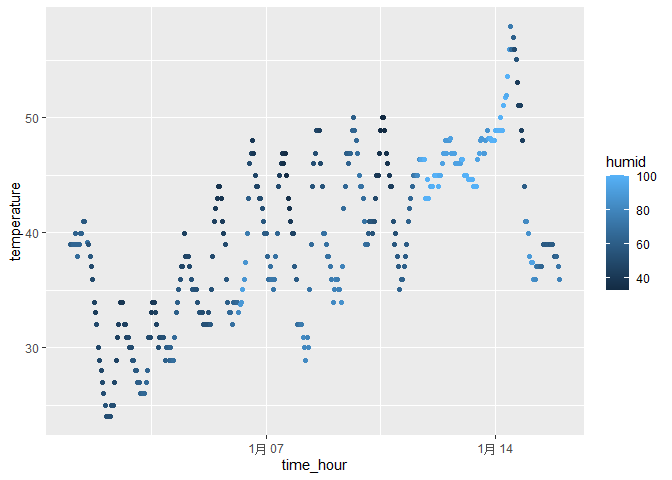
\includegraphics{p8105_hw1_yz4719_files/figure-latex/scatterplot-1.pdf}

\begin{Shaded}
\begin{Highlighting}[]
\FunctionTok{ggsave}\NormalTok{(}\StringTok{"hw1\_plot\_1.pdf"}\NormalTok{)}
\end{Highlighting}
\end{Shaded}

\begin{verbatim}
## Saving 6.5 x 4.5 in image
\end{verbatim}

\begin{verbatim}
## Warning in grid.Call(C_textBounds, as.graphicsAnnot(x$label), x$x, x$y, :
## 'mbcsToSbcs'里转换'1月 07'出错:<e6>代替了dot
\end{verbatim}

\begin{verbatim}
## Warning in grid.Call(C_textBounds, as.graphicsAnnot(x$label), x$x, x$y, :
## 'mbcsToSbcs'里转换'1月 07'出错:<9c>代替了dot
\end{verbatim}

\begin{verbatim}
## Warning in grid.Call(C_textBounds, as.graphicsAnnot(x$label), x$x, x$y, :
## 'mbcsToSbcs'里转换'1月 07'出错:<88>代替了dot
\end{verbatim}

\begin{verbatim}
## Warning in grid.Call(C_textBounds, as.graphicsAnnot(x$label), x$x, x$y, :
## 'mbcsToSbcs'里转换'1月 14'出错:<e6>代替了dot
\end{verbatim}

\begin{verbatim}
## Warning in grid.Call(C_textBounds, as.graphicsAnnot(x$label), x$x, x$y, :
## 'mbcsToSbcs'里转换'1月 14'出错:<9c>代替了dot
\end{verbatim}

\begin{verbatim}
## Warning in grid.Call(C_textBounds, as.graphicsAnnot(x$label), x$x, x$y, :
## 'mbcsToSbcs'里转换'1月 14'出错:<88>代替了dot
\end{verbatim}

\begin{verbatim}
## Warning in grid.Call(C_textBounds, as.graphicsAnnot(x$label), x$x, x$y, :
## 'mbcsToSbcs'里转换'1月 07'出错:<e6>代替了dot
\end{verbatim}

\begin{verbatim}
## Warning in grid.Call(C_textBounds, as.graphicsAnnot(x$label), x$x, x$y, :
## 'mbcsToSbcs'里转换'1月 07'出错:<9c>代替了dot
\end{verbatim}

\begin{verbatim}
## Warning in grid.Call(C_textBounds, as.graphicsAnnot(x$label), x$x, x$y, :
## 'mbcsToSbcs'里转换'1月 07'出错:<88>代替了dot
\end{verbatim}

\begin{verbatim}
## Warning in grid.Call(C_textBounds, as.graphicsAnnot(x$label), x$x, x$y, :
## 'mbcsToSbcs'里转换'1月 14'出错:<e6>代替了dot
\end{verbatim}

\begin{verbatim}
## Warning in grid.Call(C_textBounds, as.graphicsAnnot(x$label), x$x, x$y, :
## 'mbcsToSbcs'里转换'1月 14'出错:<9c>代替了dot
\end{verbatim}

\begin{verbatim}
## Warning in grid.Call(C_textBounds, as.graphicsAnnot(x$label), x$x, x$y, :
## 'mbcsToSbcs'里转换'1月 14'出错:<88>代替了dot
\end{verbatim}

\begin{verbatim}
## Warning in grid.Call(C_textBounds, as.graphicsAnnot(x$label), x$x, x$y, :
## 'mbcsToSbcs'里转换'1月 07'出错:<e6>代替了dot
\end{verbatim}

\begin{verbatim}
## Warning in grid.Call(C_textBounds, as.graphicsAnnot(x$label), x$x, x$y, :
## 'mbcsToSbcs'里转换'1月 07'出错:<9c>代替了dot
\end{verbatim}

\begin{verbatim}
## Warning in grid.Call(C_textBounds, as.graphicsAnnot(x$label), x$x, x$y, :
## 'mbcsToSbcs'里转换'1月 07'出错:<88>代替了dot
\end{verbatim}

\begin{verbatim}
## Warning in grid.Call(C_textBounds, as.graphicsAnnot(x$label), x$x, x$y, :
## 'mbcsToSbcs'里转换'1月 14'出错:<e6>代替了dot
\end{verbatim}

\begin{verbatim}
## Warning in grid.Call(C_textBounds, as.graphicsAnnot(x$label), x$x, x$y, :
## 'mbcsToSbcs'里转换'1月 14'出错:<9c>代替了dot
\end{verbatim}

\begin{verbatim}
## Warning in grid.Call(C_textBounds, as.graphicsAnnot(x$label), x$x, x$y, :
## 'mbcsToSbcs'里转换'1月 14'出错:<88>代替了dot
\end{verbatim}

\begin{verbatim}
## Warning in grid.Call(C_textBounds, as.graphicsAnnot(x$label), x$x, x$y, :
## 'mbcsToSbcs'里转换'1月 07'出错:<e6>代替了dot
\end{verbatim}

\begin{verbatim}
## Warning in grid.Call(C_textBounds, as.graphicsAnnot(x$label), x$x, x$y, :
## 'mbcsToSbcs'里转换'1月 07'出错:<9c>代替了dot
\end{verbatim}

\begin{verbatim}
## Warning in grid.Call(C_textBounds, as.graphicsAnnot(x$label), x$x, x$y, :
## 'mbcsToSbcs'里转换'1月 07'出错:<88>代替了dot
\end{verbatim}

\begin{verbatim}
## Warning in grid.Call(C_textBounds, as.graphicsAnnot(x$label), x$x, x$y, :
## 'mbcsToSbcs'里转换'1月 14'出错:<e6>代替了dot
\end{verbatim}

\begin{verbatim}
## Warning in grid.Call(C_textBounds, as.graphicsAnnot(x$label), x$x, x$y, :
## 'mbcsToSbcs'里转换'1月 14'出错:<9c>代替了dot
\end{verbatim}

\begin{verbatim}
## Warning in grid.Call(C_textBounds, as.graphicsAnnot(x$label), x$x, x$y, :
## 'mbcsToSbcs'里转换'1月 14'出错:<88>代替了dot
\end{verbatim}

\begin{verbatim}
## Warning in grid.Call(C_textBounds, as.graphicsAnnot(x$label), x$x, x$y, :
## 'mbcsToSbcs'里转换'1月 07'出错:<e6>代替了dot
\end{verbatim}

\begin{verbatim}
## Warning in grid.Call(C_textBounds, as.graphicsAnnot(x$label), x$x, x$y, :
## 'mbcsToSbcs'里转换'1月 07'出错:<9c>代替了dot
\end{verbatim}

\begin{verbatim}
## Warning in grid.Call(C_textBounds, as.graphicsAnnot(x$label), x$x, x$y, :
## 'mbcsToSbcs'里转换'1月 07'出错:<88>代替了dot
\end{verbatim}

\begin{verbatim}
## Warning in grid.Call(C_textBounds, as.graphicsAnnot(x$label), x$x, x$y, :
## 'mbcsToSbcs'里转换'1月 14'出错:<e6>代替了dot
\end{verbatim}

\begin{verbatim}
## Warning in grid.Call(C_textBounds, as.graphicsAnnot(x$label), x$x, x$y, :
## 'mbcsToSbcs'里转换'1月 14'出错:<9c>代替了dot
\end{verbatim}

\begin{verbatim}
## Warning in grid.Call(C_textBounds, as.graphicsAnnot(x$label), x$x, x$y, :
## 'mbcsToSbcs'里转换'1月 14'出错:<88>代替了dot
\end{verbatim}

\begin{verbatim}
## Warning in grid.Call(C_textBounds, as.graphicsAnnot(x$label), x$x, x$y, :
## 'mbcsToSbcs'里转换'1月 07'出错:<e6>代替了dot
\end{verbatim}

\begin{verbatim}
## Warning in grid.Call(C_textBounds, as.graphicsAnnot(x$label), x$x, x$y, :
## 'mbcsToSbcs'里转换'1月 07'出错:<9c>代替了dot
\end{verbatim}

\begin{verbatim}
## Warning in grid.Call(C_textBounds, as.graphicsAnnot(x$label), x$x, x$y, :
## 'mbcsToSbcs'里转换'1月 07'出错:<88>代替了dot
\end{verbatim}

\begin{verbatim}
## Warning in grid.Call(C_textBounds, as.graphicsAnnot(x$label), x$x, x$y, :
## 'mbcsToSbcs'里转换'1月 14'出错:<e6>代替了dot
\end{verbatim}

\begin{verbatim}
## Warning in grid.Call(C_textBounds, as.graphicsAnnot(x$label), x$x, x$y, :
## 'mbcsToSbcs'里转换'1月 14'出错:<9c>代替了dot
\end{verbatim}

\begin{verbatim}
## Warning in grid.Call(C_textBounds, as.graphicsAnnot(x$label), x$x, x$y, :
## 'mbcsToSbcs'里转换'1月 14'出错:<88>代替了dot
\end{verbatim}

\begin{verbatim}
## Warning in grid.Call(C_textBounds, as.graphicsAnnot(x$label), x$x, x$y, :
## 'mbcsToSbcs'里转换'1月 07'出错:<e6>代替了dot
\end{verbatim}

\begin{verbatim}
## Warning in grid.Call(C_textBounds, as.graphicsAnnot(x$label), x$x, x$y, :
## 'mbcsToSbcs'里转换'1月 07'出错:<9c>代替了dot
\end{verbatim}

\begin{verbatim}
## Warning in grid.Call(C_textBounds, as.graphicsAnnot(x$label), x$x, x$y, :
## 'mbcsToSbcs'里转换'1月 07'出错:<88>代替了dot
\end{verbatim}

\begin{verbatim}
## Warning in grid.Call(C_textBounds, as.graphicsAnnot(x$label), x$x, x$y, :
## 'mbcsToSbcs'里转换'1月 14'出错:<e6>代替了dot
\end{verbatim}

\begin{verbatim}
## Warning in grid.Call(C_textBounds, as.graphicsAnnot(x$label), x$x, x$y, :
## 'mbcsToSbcs'里转换'1月 14'出错:<9c>代替了dot
\end{verbatim}

\begin{verbatim}
## Warning in grid.Call(C_textBounds, as.graphicsAnnot(x$label), x$x, x$y, :
## 'mbcsToSbcs'里转换'1月 14'出错:<88>代替了dot
\end{verbatim}

\begin{verbatim}
## Warning in grid.Call(C_textBounds, as.graphicsAnnot(x$label), x$x, x$y, :
## 'mbcsToSbcs'里转换'1月 07'出错:<e6>代替了dot
\end{verbatim}

\begin{verbatim}
## Warning in grid.Call(C_textBounds, as.graphicsAnnot(x$label), x$x, x$y, :
## 'mbcsToSbcs'里转换'1月 07'出错:<9c>代替了dot
\end{verbatim}

\begin{verbatim}
## Warning in grid.Call(C_textBounds, as.graphicsAnnot(x$label), x$x, x$y, :
## 'mbcsToSbcs'里转换'1月 07'出错:<88>代替了dot
\end{verbatim}

\begin{verbatim}
## Warning in grid.Call(C_textBounds, as.graphicsAnnot(x$label), x$x, x$y, :
## 'mbcsToSbcs'里转换'1月 14'出错:<e6>代替了dot
\end{verbatim}

\begin{verbatim}
## Warning in grid.Call(C_textBounds, as.graphicsAnnot(x$label), x$x, x$y, :
## 'mbcsToSbcs'里转换'1月 14'出错:<9c>代替了dot
\end{verbatim}

\begin{verbatim}
## Warning in grid.Call(C_textBounds, as.graphicsAnnot(x$label), x$x, x$y, :
## 'mbcsToSbcs'里转换'1月 14'出错:<88>代替了dot
\end{verbatim}

\begin{verbatim}
## Warning in grid.Call(C_textBounds, as.graphicsAnnot(x$label), x$x, x$y, :
## 'mbcsToSbcs'里转换'1月 07'出错:<e6>代替了dot
\end{verbatim}

\begin{verbatim}
## Warning in grid.Call(C_textBounds, as.graphicsAnnot(x$label), x$x, x$y, :
## 'mbcsToSbcs'里转换'1月 07'出错:<9c>代替了dot
\end{verbatim}

\begin{verbatim}
## Warning in grid.Call(C_textBounds, as.graphicsAnnot(x$label), x$x, x$y, :
## 'mbcsToSbcs'里转换'1月 07'出错:<88>代替了dot
\end{verbatim}

\begin{verbatim}
## Warning in grid.Call(C_textBounds, as.graphicsAnnot(x$label), x$x, x$y, :
## 'mbcsToSbcs'里转换'1月 14'出错:<e6>代替了dot
\end{verbatim}

\begin{verbatim}
## Warning in grid.Call(C_textBounds, as.graphicsAnnot(x$label), x$x, x$y, :
## 'mbcsToSbcs'里转换'1月 14'出错:<9c>代替了dot
\end{verbatim}

\begin{verbatim}
## Warning in grid.Call(C_textBounds, as.graphicsAnnot(x$label), x$x, x$y, :
## 'mbcsToSbcs'里转换'1月 14'出错:<88>代替了dot
\end{verbatim}

\begin{verbatim}
## Warning in grid.Call(C_textBounds, as.graphicsAnnot(x$label), x$x, x$y, :
## 'mbcsToSbcs'里转换'1月 07'出错:<e6>代替了dot
\end{verbatim}

\begin{verbatim}
## Warning in grid.Call(C_textBounds, as.graphicsAnnot(x$label), x$x, x$y, :
## 'mbcsToSbcs'里转换'1月 07'出错:<9c>代替了dot
\end{verbatim}

\begin{verbatim}
## Warning in grid.Call(C_textBounds, as.graphicsAnnot(x$label), x$x, x$y, :
## 'mbcsToSbcs'里转换'1月 07'出错:<88>代替了dot
\end{verbatim}

\begin{verbatim}
## Warning in grid.Call(C_textBounds, as.graphicsAnnot(x$label), x$x, x$y, :
## 'mbcsToSbcs'里转换'1月 14'出错:<e6>代替了dot
\end{verbatim}

\begin{verbatim}
## Warning in grid.Call(C_textBounds, as.graphicsAnnot(x$label), x$x, x$y, :
## 'mbcsToSbcs'里转换'1月 14'出错:<9c>代替了dot
\end{verbatim}

\begin{verbatim}
## Warning in grid.Call(C_textBounds, as.graphicsAnnot(x$label), x$x, x$y, :
## 'mbcsToSbcs'里转换'1月 14'出错:<88>代替了dot
\end{verbatim}

\begin{verbatim}
## Warning in grid.Call(C_textBounds, as.graphicsAnnot(x$label), x$x, x$y, :
## 'mbcsToSbcs'里转换'1月 07'出错:<e6>代替了dot
\end{verbatim}

\begin{verbatim}
## Warning in grid.Call(C_textBounds, as.graphicsAnnot(x$label), x$x, x$y, :
## 'mbcsToSbcs'里转换'1月 07'出错:<9c>代替了dot
\end{verbatim}

\begin{verbatim}
## Warning in grid.Call(C_textBounds, as.graphicsAnnot(x$label), x$x, x$y, :
## 'mbcsToSbcs'里转换'1月 07'出错:<88>代替了dot
\end{verbatim}

\begin{verbatim}
## Warning in grid.Call(C_textBounds, as.graphicsAnnot(x$label), x$x, x$y, :
## 'mbcsToSbcs'里转换'1月 14'出错:<e6>代替了dot
\end{verbatim}

\begin{verbatim}
## Warning in grid.Call(C_textBounds, as.graphicsAnnot(x$label), x$x, x$y, :
## 'mbcsToSbcs'里转换'1月 14'出错:<9c>代替了dot
\end{verbatim}

\begin{verbatim}
## Warning in grid.Call(C_textBounds, as.graphicsAnnot(x$label), x$x, x$y, :
## 'mbcsToSbcs'里转换'1月 14'出错:<88>代替了dot
\end{verbatim}

\begin{verbatim}
## Warning in grid.Call(C_textBounds, as.graphicsAnnot(x$label), x$x, x$y, :
## 'mbcsToSbcs'里转换'1月 07'出错:<e6>代替了dot
\end{verbatim}

\begin{verbatim}
## Warning in grid.Call(C_textBounds, as.graphicsAnnot(x$label), x$x, x$y, :
## 'mbcsToSbcs'里转换'1月 07'出错:<9c>代替了dot
\end{verbatim}

\begin{verbatim}
## Warning in grid.Call(C_textBounds, as.graphicsAnnot(x$label), x$x, x$y, :
## 'mbcsToSbcs'里转换'1月 07'出错:<88>代替了dot
\end{verbatim}

\begin{verbatim}
## Warning in grid.Call(C_textBounds, as.graphicsAnnot(x$label), x$x, x$y, :
## 'mbcsToSbcs'里转换'1月 14'出错:<e6>代替了dot
\end{verbatim}

\begin{verbatim}
## Warning in grid.Call(C_textBounds, as.graphicsAnnot(x$label), x$x, x$y, :
## 'mbcsToSbcs'里转换'1月 14'出错:<9c>代替了dot
\end{verbatim}

\begin{verbatim}
## Warning in grid.Call(C_textBounds, as.graphicsAnnot(x$label), x$x, x$y, :
## 'mbcsToSbcs'里转换'1月 14'出错:<88>代替了dot
\end{verbatim}

\begin{verbatim}
## Warning in grid.Call(C_textBounds, as.graphicsAnnot(x$label), x$x, x$y, :
## 'mbcsToSbcs'里转换'1月 07'出错:<e6>代替了dot
\end{verbatim}

\begin{verbatim}
## Warning in grid.Call(C_textBounds, as.graphicsAnnot(x$label), x$x, x$y, :
## 'mbcsToSbcs'里转换'1月 07'出错:<9c>代替了dot
\end{verbatim}

\begin{verbatim}
## Warning in grid.Call(C_textBounds, as.graphicsAnnot(x$label), x$x, x$y, :
## 'mbcsToSbcs'里转换'1月 07'出错:<88>代替了dot
\end{verbatim}

\begin{verbatim}
## Warning in grid.Call(C_textBounds, as.graphicsAnnot(x$label), x$x, x$y, :
## 'mbcsToSbcs'里转换'1月 14'出错:<e6>代替了dot
\end{verbatim}

\begin{verbatim}
## Warning in grid.Call(C_textBounds, as.graphicsAnnot(x$label), x$x, x$y, :
## 'mbcsToSbcs'里转换'1月 14'出错:<9c>代替了dot
\end{verbatim}

\begin{verbatim}
## Warning in grid.Call(C_textBounds, as.graphicsAnnot(x$label), x$x, x$y, :
## 'mbcsToSbcs'里转换'1月 14'出错:<88>代替了dot
\end{verbatim}

\begin{verbatim}
## Warning in grid.Call.graphics(C_text, as.graphicsAnnot(x$label), x$x, x$y, :
## 'mbcsToSbcs'里转换'1月 07'出错:<e6>代替了dot
\end{verbatim}

\begin{verbatim}
## Warning in grid.Call.graphics(C_text, as.graphicsAnnot(x$label), x$x, x$y, :
## 'mbcsToSbcs'里转换'1月 07'出错:<9c>代替了dot
\end{verbatim}

\begin{verbatim}
## Warning in grid.Call.graphics(C_text, as.graphicsAnnot(x$label), x$x, x$y, :
## 'mbcsToSbcs'里转换'1月 07'出错:<88>代替了dot
\end{verbatim}

\begin{verbatim}
## Warning in grid.Call.graphics(C_text, as.graphicsAnnot(x$label), x$x, x$y, :
## 'mbcsToSbcs'里转换'1月 07'出错:<e6>代替了dot
\end{verbatim}

\begin{verbatim}
## Warning in grid.Call.graphics(C_text, as.graphicsAnnot(x$label), x$x, x$y, :
## 'mbcsToSbcs'里转换'1月 07'出错:<9c>代替了dot
\end{verbatim}

\begin{verbatim}
## Warning in grid.Call.graphics(C_text, as.graphicsAnnot(x$label), x$x, x$y, :
## 'mbcsToSbcs'里转换'1月 07'出错:<88>代替了dot
\end{verbatim}

\begin{verbatim}
## Warning in grid.Call.graphics(C_text, as.graphicsAnnot(x$label), x$x, x$y, :
## 'mbcsToSbcs'里转换'1月 14'出错:<e6>代替了dot
\end{verbatim}

\begin{verbatim}
## Warning in grid.Call.graphics(C_text, as.graphicsAnnot(x$label), x$x, x$y, :
## 'mbcsToSbcs'里转换'1月 14'出错:<9c>代替了dot
\end{verbatim}

\begin{verbatim}
## Warning in grid.Call.graphics(C_text, as.graphicsAnnot(x$label), x$x, x$y, :
## 'mbcsToSbcs'里转换'1月 14'出错:<88>代替了dot
\end{verbatim}

\begin{verbatim}
## Warning in grid.Call.graphics(C_text, as.graphicsAnnot(x$label), x$x, x$y, :
## 'mbcsToSbcs'里转换'1月 14'出错:<e6>代替了dot
\end{verbatim}

\begin{verbatim}
## Warning in grid.Call.graphics(C_text, as.graphicsAnnot(x$label), x$x, x$y, :
## 'mbcsToSbcs'里转换'1月 14'出错:<9c>代替了dot
\end{verbatim}

\begin{verbatim}
## Warning in grid.Call.graphics(C_text, as.graphicsAnnot(x$label), x$x, x$y, :
## 'mbcsToSbcs'里转换'1月 14'出错:<88>代替了dot
\end{verbatim}

\hypertarget{question-2}{%
\section{Question 2:}\label{question-2}}

\begin{Shaded}
\begin{Highlighting}[]
\NormalTok{sample\_2 }\OtherTok{=} \FunctionTok{tibble}\NormalTok{(}
  \AttributeTok{samp =} \FunctionTok{rnorm}\NormalTok{(}\DecValTok{10}\NormalTok{),}
  \AttributeTok{vec\_logical =}\NormalTok{ samp }\SpecialCharTok{\textgreater{}} \DecValTok{0}\NormalTok{,}
  \AttributeTok{vec\_char =} \FunctionTok{c}\NormalTok{(}\StringTok{"my"}\NormalTok{, }\StringTok{"name"}\NormalTok{, }\StringTok{"is"}\NormalTok{, }\StringTok{"samantha"}\NormalTok{, }\StringTok{"and"}\NormalTok{, }\StringTok{"this"}\NormalTok{, }\StringTok{"should"}\NormalTok{, }\StringTok{"be"}\NormalTok{, }\StringTok{"ten"}\NormalTok{, }\StringTok{"words"}\NormalTok{),}
  \AttributeTok{vec\_factor =} \FunctionTok{factor}\NormalTok{(}\FunctionTok{c}\NormalTok{(}\StringTok{"elder"}\NormalTok{, }\StringTok{"youth"}\NormalTok{, }\StringTok{"middle age"}\NormalTok{, }\StringTok{"elder"}\NormalTok{, }\StringTok{"teen"}\NormalTok{, }\StringTok{"middle age"}\NormalTok{, }\StringTok{"youth"}\NormalTok{, }\StringTok{"middle age"}\NormalTok{, }\StringTok{"teen"}\NormalTok{, }\StringTok{"youth"}\NormalTok{ ))}
\NormalTok{  )}
\end{Highlighting}
\end{Shaded}

\hypertarget{means}{%
\section{means}\label{means}}

\begin{Shaded}
\begin{Highlighting}[]
\NormalTok{random\_mean }\OtherTok{=} \FunctionTok{mean}\NormalTok{(}\FunctionTok{pull}\NormalTok{(sample\_2, samp))}
\NormalTok{logical\_mean }\OtherTok{=} \FunctionTok{mean}\NormalTok{(}\FunctionTok{pull}\NormalTok{(sample\_2, vec\_logical))}
\NormalTok{char\_mean }\OtherTok{=} \FunctionTok{mean}\NormalTok{(}\FunctionTok{pull}\NormalTok{(sample\_2, vec\_char))}
\end{Highlighting}
\end{Shaded}

\begin{verbatim}
## Warning in mean.default(pull(sample_2, vec_char)):
## 参数不是数值也不是逻辑值:回覆NA
\end{verbatim}

\begin{Shaded}
\begin{Highlighting}[]
\NormalTok{factor\_mean }\OtherTok{=} \FunctionTok{mean}\NormalTok{(}\FunctionTok{pull}\NormalTok{(sample\_2, vec\_factor))}
\end{Highlighting}
\end{Shaded}

\begin{verbatim}
## Warning in mean.default(pull(sample_2, vec_factor)):
## 参数不是数值也不是逻辑值:回覆NA
\end{verbatim}

\end{document}
